% !TEX root = ../build-polygon/proof-recursion.tex


%%%%%%%%%%%%%%%%%%%%%%%%%%%%%%%%%%%%%%%%%%%%%%%%%%%%%%%%%%%%%%%
\section{Tools}

\subsection{PIL}

Polynomial Identity Language (PIL) is a novel domain-specific language to define the constraints of computation traces of either computations based on the circuit model or computations based on the state machine model. 
The constraints of the zkEVM execution trace, which is based on a state machine, are specified with PIL.


\subsection{Circom}

In Figure \ref{fig:circom_architecture} we show the architecture of Circom.
Programmers can use the Circom language to define arithmetic circuits and the compiler generates a file with the set of associated R1CS constraints together with a program (written either in cpp or wasm) that can be run to efficiently compute a valid assignment to all wires of the circuit.

After compiling a circuit, we can calculate all the signals that match the set of constraints of the circuit using the cpp or wasm programs generated by the compiler. To do so, we simply need to provide a file with a set of valid input values, and the program will calculate a set of values for the rest of signals of the circuit. A valid set of input, intermediate and output values is called \textit{witness}.

\begin{figure}[H]
\centering
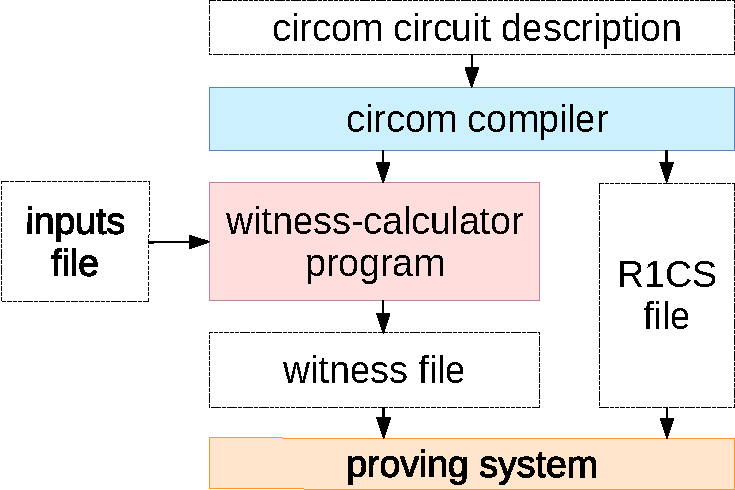
\includegraphics[width=0.5\textwidth]{\recursiondir/figures/circom-architecture}
\caption{Circom}
\label{fig:circom_architecture}
\end{figure}



\subsection{Non-recursive STARK \label{subsec:non_recursive_STARK}}

The setting for STARK proofs are machine-like computations from which we can derive a certain arithmetization, 
giving us a set of constraints describing its correct execution. 
The polynomial building the constraints that arise from a certain arithmetization can, 
in fact, depend on the inputs of the state machine itself giving what we call \textit{committed polynomials} and, 
by definition, should be computed once per proof. 
However, a polynomial that is completely independent of the input values so it is kept constant among several executions of the same state machine should be computed only once per arithmetization. 
The former kind of polynomials are called \textit{constant polynomials} and represent the computation that is being executed, so that they are publicly available for both the prover and the verifier, unlike the committed ones, which are not directly available to the verifier.


\begin{figure}[H]
\centering
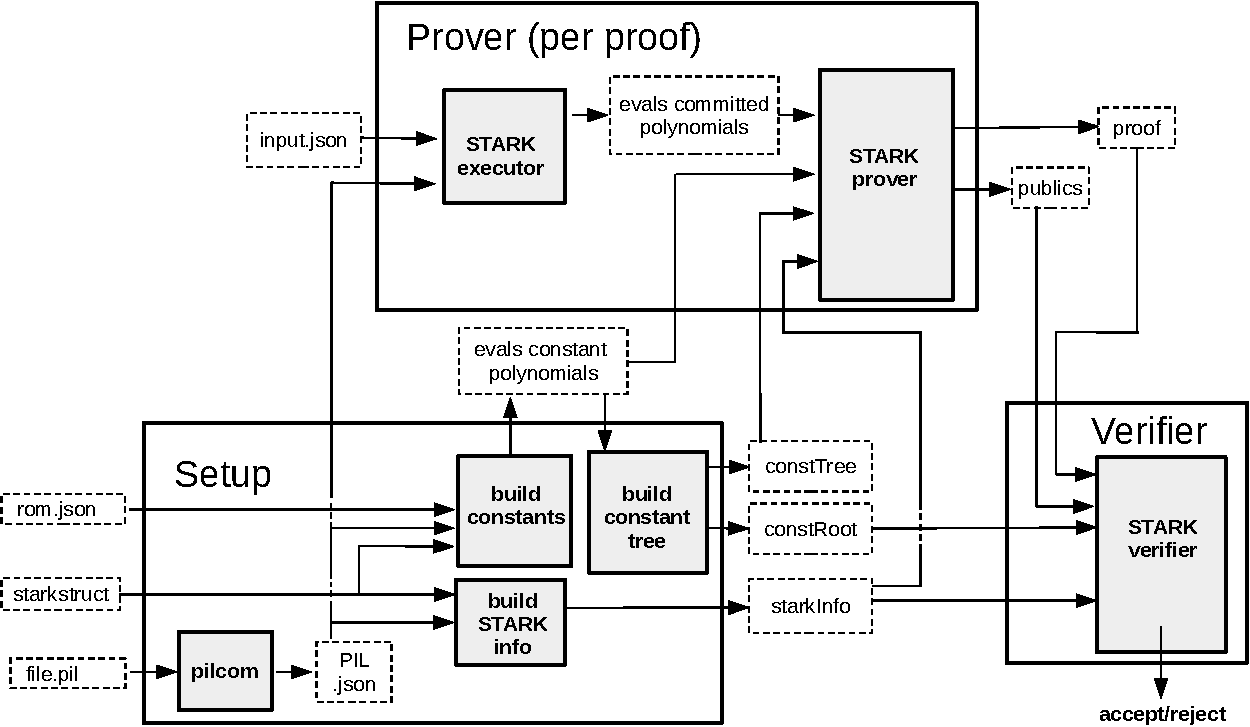
\includegraphics[width=\textwidth]{\recursiondir/figures/pil-stark-no_recursive-blocks}
\caption{Non recursive STARK.}
\label{fig:non-recursive}
\end{figure}

Due to the fact that all the constant polynomials do not depend on the particular inputs of a certain computation executed by the state machine, we can split the processes that make up the generation of a proof in two: the \textit{setup phase} and the \textit{proving phase}. 
This allows to execute both processes separately, which is highly important in order not to execute the constants' computation per proof, drastically increasing the proving time. 

The \textit{setup phase} performs all the pre-processing. 
The setup is only done once per state machine definition, allowing to reuse it whether the definition does not change. 
The definition of a state machine with \texttt{pil-stark} has three parts:

\begin{compactitem}
\item The \texttt{rom.json} file to build the computation.
\item The configuration of the FRI used in the STARK proof, inside a \texttt{starkstruct} file, specifying the blowup factor, the size of the trace and its LDE (Low Degree Extension) and the number of queries to be performed.
\item The \texttt{PIL} description of the STARK state machine, that is to say, the constraints that define the correctness of the execution trace (\texttt{file.pil} file).
\end{compactitem}

The PIL file and the \texttt{starkstruct} are used by the \texttt{build STARK info} process to write a file called \texttt{starkInfo} containing, apart from all the FRI-related parameters, several useful fields related with the PIL and the shape of the constraints. The PIL description is parsed with a compiler called \texttt{pilcom}\footnote{The \texttt{pilcom} parser is written with \url{https://github.com/zaach/jison}, which generates bottom-up parsers in JavaScript.} to obtain a parsed JSON version of the PIL, which will be used by the prover to compute all the polynomials involved in the proving procedure. The \texttt{build constants} process, using the parsed PIL, computes the evaluations of the constant polynomials over the evaluation domain determined by the \texttt{starkstruct}. Additionally, once this evaluations are computed, the \texttt{build constant tree} process generates the Merkle root of its corresponding tree for the verifier, which we call constant root (\texttt{constRoot}). 

In the \textit{proving phase}, the Prover executes all the processes that, given an input, generate a proof for the computation. 
The STARK executor process computes the evaluations of the polynomials that are going to be committed. To do so, it takes the names and descriptions of the polynomials from the parsed PIL and the provided inputs. Observe that, since the values of the committed polynomials are strongly dependent on the inputs, this procedure should be executed once per proof, unlike the setup phase. 

Finally, the \texttt{pil-stark} STARK prover process takes the evaluations of both the constant and the committed polynomials of the previous steps and all the information stored in the \texttt{starkInfo} object in order to generate the corresponding STARK proof and the associated public values for which the proof is valid. 
We use the \textsf{eSTARK} protocol, which is specially designed to proof PIL statements. 
The \textsf{eSTARK} protocol is composed on two main stages:

\begin{itemize}
\item \textit{Low-Degree Reduction phase}: Following \cite{EPRINT:StarkWare21}, first of all, we obtain a polynomial called FRI which codifies the validity of the values of the trace according to the PIL into the fact that it has low degree. This polynomial is committed to the verifier, as well as several previous polynomials that are used to provide consistency checks between them.  This phase, however, differs from the one described in \cite{EPRINT:StarkWare21} because PIL also accepts, apart from polynomial equalities, arguments such lookups, permutations or even copy-constraints (called connection arguments). Hence, this phase needs to be adapted in order to proof the correctness of each of the enumerated arguments. This serves as a motivation to call this protocol \textsf{eSTARK}, standing for \textit{extended STARK}. 

\item \textit{FRI phase}: After obtaining the so called FRI polynomial, the prover and the verifier are involved into a FRI Protocol \cite{ICALP:BBHR18}, aiming for proving that the committed polynomial has low degree (more concretely, it proves that the committed values of the polynomials raise a function that is close enough to a polynomial of low degree, see \cite{ICALP:BBHR18} for more information on FRI Protocol). 
\end{itemize}

The first stage can, in turn, be divided into several rounds. Below, we describe in a high level what is each of the rounds aiming.

\begin{itemize}

\item \textit{Round 1:} Given the trace column polynomials interpolating the execution trace, the prover commits to them.

\item \textit{Round 2:} The prover commits, for each lookup argument, to the $h$-polynomials of the modified \plookup version described in \cite{EPRINT:PFMBM22} (see \cite{EPRINT:GabWil20} for more information about \plookup protocol).

\item \textit{Round 3:} The prover commits to the grand-product polynomials for each of the arguments appearing in the PIL together with some intermediate polynomials used to reduce the degree of the grand products. This is due to the fact that \texttt{pil-stark} imposes a degree bound when committing to a polynomial. See \cite{EPRINT:GabWilCio19, EPRINT:GabWil20} for the specification of the grand-products of each of the different arguments allowed in PIL.

\item \textit{Round 4:} The prover commits to the $2$ polynomials $Q_1, Q_2$ arising from the splitting of the quotient polynomial $Q$. 

\item \textit{Round 5:} The prover provides the verifier with all the necessary evaluations of the polynomials so that he/she can execute the corresponding checks. 

\item \textit{Round 6:} The prover receives two randomness from the verifier which are used to construct the previously described FRI polynomial. Then, the prover and the verifier are involved into a FRI Protocol, ending with the prover sending the corresponding FRI proof to the verifier. 

\end{itemize} 


After the proof is generated, it is sent to the Verifier instance so that he/she can start the verification procedure, after what will accept or reject the proof. 



%%%%%%%%%%%%%%%%%%%%%%%%%%%%%%%%%%%%%%%%%%%%%%%%%%%%%%%%%%%%%%%
\section{Composition, Recursion and Aggregation}

\subsection{Composition}

As shown in Section \ref{subsec:non_recursive_STARK}, the basic verification of a STARK is performed by a verifier entity using the proof, the publics and some other verifier parameters.
Composing proofs means using different proving systems together to generate a proof.
Generally composition is used to increase the efficiency of some part of the system.
In our case, as first proving system we use a STARK and our main idea of composition is to delegate the verification procedure of the STARK proof $\pi_{STARK}$ to a verification circuit $C$.
In this case, if the prover provides a proof for the correct execution of the verification circuit $\pi_{CIRCUIT}$, then this is enough to verify the original STARK.
As shown in Figure \ref{fig:simple-composition}, in this case, 
the verifier entity just verifies the proof of the STARK verification circuit $\pi_{CIRCUIT}$.
The advantage of this composition is that $\pi_{CIRCUIT}$ is smaller and faster to verify than $\pi_{STARK}$.

\begin{figure}[H]
\centering
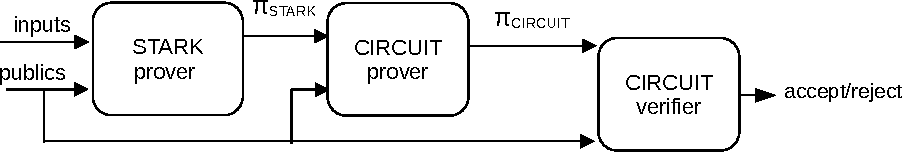
\includegraphics[width=0.7\textwidth]{\recursiondir/figures/simple-composition}
\caption{Simple composition.}
\label{fig:simple-composition}
\end{figure}
